% arara: pdflatex
% arara: biber
% arara: makeindex
% arara: nomencl
% arara: pdflatex
% arara: pdflatex

\documentclass[a4paper,12pt]{article}
%\RequirePackage[l2tabu,orthodox]{nag}

\usepackage{upreport}
\addbibresource{report_actual.bib}
\title{Integrated Heat Pump/Organic Rankine Cycle System for Waste Heat Recovery}
\author{Carsten Rembold}
\studentnumber{16052481}
\subject{CSC 411}
\date{\today}

%Nomenclature unit command
\newcommand{\nomunit}[1]{%
\renewcommand{\nomentryend}{\hspace*{\fill}#1}}
\usepackage[colorinlistoftodos, color = lime]{todonotes}
% Create a custom user command or run the following 
%  makeindex %.nlo -s nomencl.ist -o %.nls
% execute this command after compiling your file once, then compile a second time to generate a nomenclature table

\begin{document}
\maketitle
\makecoverpage

\pagestyle{plain}
\thispagestyle{plain}
\pagenumbering{roman}

\begin{center}
\LARGE\textbf{\thetitle}
\end{center}

\section*{Abstract}
\addcontentsline{toc}{section}{Abstract}%
A comparison of differing simulation platforms for a waste heat recovery system is completed. This is with specific reference to the Integrated heat pump/organic Rankine cycle system. The comparison is directly within the bounds of the simulation system and does not include any optimisation improvements. The comparison is carried out with the goal of comparing free and expensive software. Information is gathered with regards to the system to allow for simulation of the system.

Keywords: integrated ORC, waste heat, energy recovery.
\setcounter{page}{3}

\newpage
\tableofcontents

\iftotalfigures%
\newpage%
\listoffigures%
\fi

\iftotaltables%
\newpage%
\listoftables%
\fi

\newpage

%\chapter*{Nomenclature}
\printnomenclature
\newpage

\pagestyle{plain}
\setcounter{page}{1}
\pagenumbering{arabic}

% Note: To edit the abstract, edit the file abstract.tex

\section{Introduction}
The presence of continually increasing energy costs has resulted in a major increase in the interest of energy saving measures. Energy losses through heat is a big problem on most industrial sites, with waste heat not being recovered. This has led to the implementation of technology in an attempt to capture a portion of waste heat in a usable form. The conversion of heat into electricity occurs in a cyclic process known as a heat engine. Commonly heat engines use water as an operating fluid. New technology, known as an organic Rankine cycle (ORC), suggests the use of organic fluids as the working fluid in the heat engine to improve waste heat recovery. 

Organic Rankine cycles have the advantage of recovering heat from a low-temperature waste heat source. The negative side is that ORC's have low efficiencies due to a mismatch in the thermal profiles of the waste heat and the organic working fluid. \textcite{YU2018330} suggests, with evidence of simulation, that with the introduction of heat to the ORC the pinch points (thermal limitations) may be alleviated, thereby increasing the efficiency of the system. \textcite{YU2018330} make use of ``Aspen Plus" to provide results for the investigation carried out. The use of ``Aspen Plus" is the focus of the investigation to be carried out

Expensive software such as ``Aspen Plus" currently have control over process simulation. These tools, though greatly assistive in student learning, provide poor long-term usefulness as most companies refuse to pay for the expensive software. The expensive software also tends to be more complex (multi-functional). Cheaper, more simplistic software could offer a better alternative for learning and long-term use. 

The aim of this project is to replicate the results obtained by \textcite{YU2018330} with the free software package "Anaconda", using the Python language, in combination with the properties package ``Coolprop'', \parencite{Coolprop}, in order to determine whether or not it is possible to achieve similar results with free software as with expensive software. A secondary goal is to build capacity within the chemical engineering department at the University of Pretoria for the use of free software in promoting long-term use for students.

The system used in \textcite{YU2018330} is to be modelled. Each individual component is modelled for a standalone organic Rankine cycle. Results for the standalone ORC are to be matched with \textcite{YU2018330}. The heat pump is then modelled and integrated with the standalone ORC and compared with the base paper results. The optimisation of the integration routine used in determining thermal suitability is excluded.

\newpage
\section{Theory}

\subsection{Waste Heat}

Chemical plants make use of large quantities of heat and power. There is power needed for motors, pumps, instrumentation and numerous other uses. Commonly this power is sourced through an external electricity company which creates additional operating costs \parencite{Kemp2007}. The issue is that this power is essential for plant operation. Plants making use of steam heating, flue gases and any assortment of fluids that are above ambient temperature all have heat sources. Each heat source contains thermal energy that can be recovered and converted to power. Even though this recovery always has poor efficiency \parencite{ShaumThermo}, the reclaiming of thousands of Watts of energy for re-use in a plant makes this a desirable option, especially with decreasing energy supplies and increasing energy costs \parencite{Kemp2007}.  

\textcite{BCS2008} suggests that between 20 and \SI{50}{\%} of heat entering industrial systems is lost as waste heat, in the context of vast energy amounts, this is an appreciable loss. The heat losses have a major impact on plant energy costs in the short-termand on the environment in the long-term. The main factors that are known to impact the ability for implementation of a waste heat recovery system are: heat quantity, waste heat temperature, waste stream composition, minimum allowable temperature and economies of scale \parencite{BCS2008}. These factors will need to be considered if a feasible heat recovery system is to be investigated. Feasibility at this stage is not considered so further explanation has been left out.
\subsection{Thermodynamic Cycles}

\subsubsection{Heat Engines}
\label{sec:Heat&Pump}

Heat engines are most commonly used as waste heat recovery systems. The most basic form of a heat engine is high-pressure steam which is passed over the blades of a turbine.  The turbine causes the rotation of a shaft which produces work (commonly electricity); this results in a large pressure drop and hence low-pressure steam exits the turbine. This concept is adapted into the cyclic process of the heat engine. The premise of this cycle is the addition of heat at a high temperature and release of heat at a low temperature leading to the output of usable work \parencite{SmithVanNessAbbott}. Figure \ref{fig:BasicORC} displays a basic heat engine with its key components and features.
 
 \begin{figure}[htbp]
  \centering
  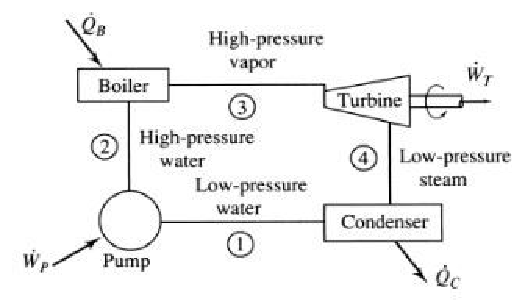
\includegraphics[scale = 0.8]{Images/Basic_Cycle.pdf}
  \caption{Basic Rankine cycle \parencite{ShaumThermo}.}
  \label{fig:BasicORC}
\end{figure}

\nomenclature{$\eta_T$}{Thermal efficiency \nomunit{1}}Thermal efficiency $\eta_T$ determines the effectiveness of a heat engine as per Equation \ref{eq:ThermalEffec}. The efficiency is the ratio of the net work $W$ \nomenclature{W}{Net Work \nomunit{\si{\kilo\joule}}} to the heat absorbed $Q_H$ \nomenclature{$Q_H$}{Heat absorbed \nomunit{\si{\kilo\joule}}}.

\begin{equation}
    \label{eq:ThermalEffec}
    \eta_T = \frac{|W|}{|Q_H|} = \frac{|Q_H|-|Q_C|}{|Q_H|} = 1-\frac{|Q_C|}{|Q_H|}
\end{equation}

To achieve 100 \% efficiency it is necessary for the heat rejected $Q_C$ \nomenclature{$Q_C$}{Heat rejected \nomunit{\si{\kilo\joule}}} to equal zero, which implies that the cold reservoir temperature must be zero – this is currently unachievable \parencite{SmithVanNessAbbott}. According to \textcite{Kemp2007}, heat engines operate at a maximum of 40 \% thermal efficiency which appears to be an unexpectedly low efficiency. \citet{ShaumThermo} describes the Carnot (ideal) cycle which explains this phenomenon. The Carnot cycle operates under the following ideal assumptions:

\begin{itemize}
    \item Isothermal compression and expansion
    \item Isentropic reversible compression and expansion
    \item The pump and turbine can operate at saturated liquid and vapour limits
\end{itemize}

\textcite{Chang2014} show that the assumptions above condense $\eta_T$ into Equation \ref{eq:CarnotEffic} known as the Carnot efficiency $\eta_c$\nomenclature{$\eta_c$}{Carnot efficiency \nomunit{1}}. Carnot efficiency is the maximum efficiency that can be achieved irrespective of fluid type and is only dependant on the cold reservoir temperature $T_C$\nomenclature{$T_C$}{Temperature of cold reservoir \nomunit{\si{\celsius}}} and the hot reservoir temperature $T_H$\nomenclature{$T_H$}{Temperature of hot reservoir \nomunit{\si{\celsius}}}.

\begin{equation}
    \label{eq:CarnotEffic}
    \eta_{c} = 1 - \frac{T_C}{T_H}
\end{equation}

This shows that all heat engines are limited by the Carnot efficiency. This limitation is important as the thermal efficiencies achieved by realisable systems should to that placed in the context of the maximum possible efficiency of that system \parencite{Chang2014}.

\subsubsection{Heat Pumps}
 There exists multiple forms of heat pumps including vapour refrigeration, absorption refrigeration and gas refrigeration. The vapour compression refrigeration (VCR) cycle is easy to implement practically and is diverse over a large range of heat pump sizes and applications \parencite{ShaumThermo}. The VCR cycle is what will be considered for the rest of this report. The VCR cycle contains a working fluid which is most commonly some form of refrigerant. The principles on which a heat pump operates is the rejection of heat at high pressure and temperature and the addition of heat at low pressure and temperature \parencite{SmithVanNessAbbott}.

A heat pump in its goal is the reverse of a heat engine. The goal is to take heat from a low temperature source and with the addition of work to release this at a higher temperature known as "upgrading" the heat source \parencite{Kemp2007}. The Rankine cycle is adjusted as follows: The fluid flow direction is reversed, the turbine is replaced with a compressor, and the pump is replaced with a throttling valve. Figure \ref{fig:HeatPump} shows a form of the heat pump known as a Vapour Compression Refrigeration (VCR) cycle.

\begin{equation}
    \label{eq:COP}
    COP_{hp} = \frac{|Q_{out}|}{|W_{in}|}
\end{equation}

 The effectivity of a heat engine may be expressed as the coefficient of performance $COP$\nomenclature{COP}{Coefficient of performance \nomunit{1}} which is simply the inverse of the efficiency. The larger the $COP$ the better the ability of the heat pump to transform the work into heat \parencite{ShaumThermo}. The higher the $COP$ the less work that is required into the system and therefore the lower the operating cost of the heat pump. This measure is influenced by the working fluid used \parencite{Kemp2007}, hence the interest in discovering new refrigerants.

 \begin{figure}[htbp]
  \centering
  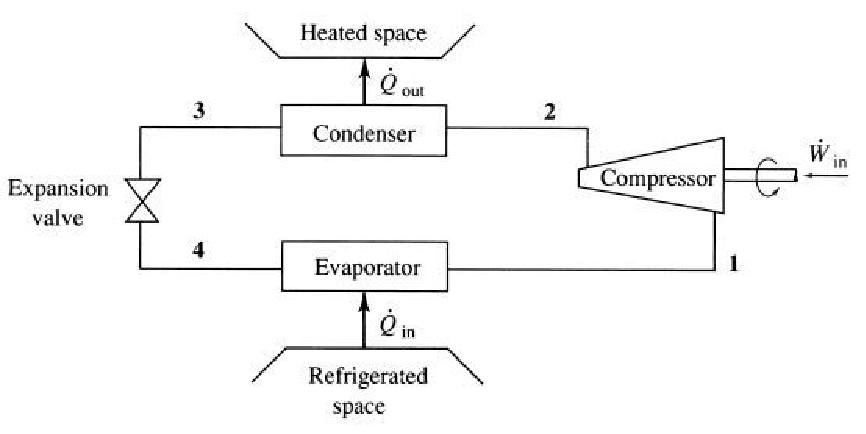
\includegraphics[scale = 0.8]{Images/Heat_Pump.pdf}
  \caption{Basic VCR cycle \parencite{ShaumThermo}.}
  \label{fig:HeatPump}
\end{figure}

\subsubsection{Organic Rankine Cycle}
Low temperature (60 - \SI{200}{\celsius}) or low-grade heat is often directly lost to the environment and is not recovered leading to thermal pollution \parencite{MagoChamraSomayaji}. The low temperature results in low efficiencies as per the Carnot efficiency, Equation \ref{eq:CarnotEffic}, \parencite{RoyMishraMisra}. Due to the low temperature of the heat source, it becomes necessary to use organic fluids as the working fluid in the Rankine cycle instead of a gas or water fluid. The purpose of the replacement is meant to increase the thermodynamic efficiency by better matching the thermal profiles of the fluid with the waste heat source \parencite{MacchiEnnio}. According to \textcite{GuWengZheng} organic fluids at low temperatures have the advantages of: high efficiencies, simple turbines and no emissions of exhaust gases amongst others. The higher efficiency of organic fluids leads to the waste heat recovery system becoming economically feasible where steam at its lower efficiency would not be \parencite{MagoChamraSomayaji}.

Organic Rankine cycles are exact replicas of a normal Rankine cycle with the exception of the use of an organic fluid as the working fluid. This means that the system is still constrained by isentropic efficiencies \parencite{MacchiEnnio}. Fluid selection is the main discussion point in terms of Rankine cycles. The fluids are categorised into three types namely: isentropic, dry, and wet \parencite{GuWengZheng}.

\subsection{Pinch Points}
\label{sec:PinchPoints}
It is necessary to delve deeper into pinch analysis prior to the integrated ORC, as the concept behind the integrated ORC is based on manipulation of pinch point. Pinch points are where the heat transfer between multiple flowing streams is limited by the minimum temperature of approach $\Delta T_{min}$\nomenclature{$\Delta T_{min}$}{Minimum temperature of approach \nomunit{\si{\celsius}}} \parencite{Kemp2007}. These pinch points occur due to the different heat bearing capacities of the streams (Heat capacities, Latent heats of evaporation and flow rates). The differing energy uptake or release rates cause a difference in the change in energy per degree change in temperature. This concept is best illustrated as per the T-H diagram Figure \ref{fig:T_H} below \parencite{Kemp2007}. The pinch point occurs at \SI{125}{\celsius} this is due to the $\Delta~T_{min}$ limitation. No further heat transfer will occur beyond this temperature and as can be seen this means that the heat transfer is limited.
 \begin{figure}[H]
  \centering
  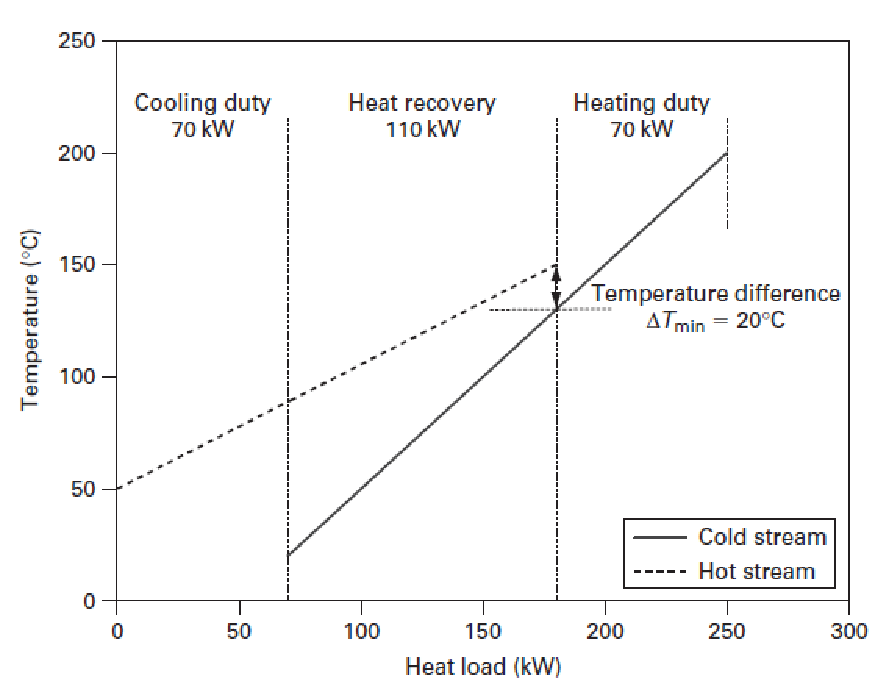
\includegraphics[scale = 0.7]{Images/T_H.pdf}
  \caption{T-H diagram with $\Delta T_{min} = $ 20  \parencite{Kemp2007}.}
  \label{fig:T_H}
\end{figure}

Figure \ref{fig:T_H} shows the convergence of the streams and the limitations of heat recovery imposed by the pinch point. In the instance of Figure \ref{fig:T_H} the pinch point occurs at \SI{130}{\celsius}. As is seen in the figure, no further heat can be transferred thus limiting the waste heat recovery. This makes pinch analysis an important factor when considering the implementation of waste heat recovery systems.

\subsection{Integrated Organic Rankine Cycle}
The integrated ORC is a combination of a heat pump and an organic Rankine cycle as per Figure \ref{fig:intORC}. The concept behind the application of an integrated ORC over a standalone ORC is directly linked to thermal pinch points and thermal composition curves as per Section \ref{sec:PinchPoints} \parencite{YU2018330}. Standalone ORC's have low conversions due to a poor match between the thermal composition curves of the waste heat source and the working fluid \parencite{MacchiEnnio}. 

 \begin{figure}[H]
  \centering
  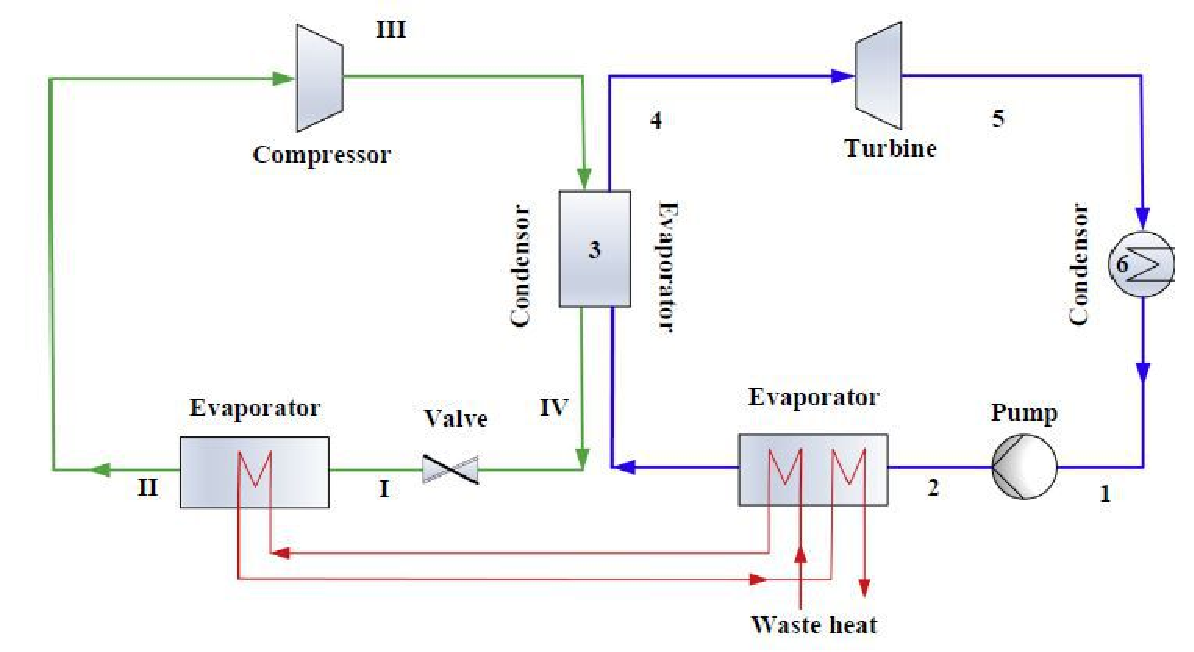
\includegraphics[scale = 0.65]{Images/IntORC.pdf}
  \caption{Integrated organic Rankine cycle \parencite{YU2018330}.}
  \label{fig:intORC}
\end{figure}

\textcite{YU2018330} shows that by increasing or upgrading the waste heat, the pinch points are alleviated thereby increasing the efficiency of the ORC. This means that the small addition in energy from the heat pump leads to a greater addition in waste heat recovery. Another explanation is that the minor addition of work in the compressor of the heat pump leads to a greater output of work from the turbine of the ORC. Figure \ref{fig:PinchPointOpt} shows the relation between pinch points and the heat transfer upgrade.

 \begin{figure}[H]
  \centering
  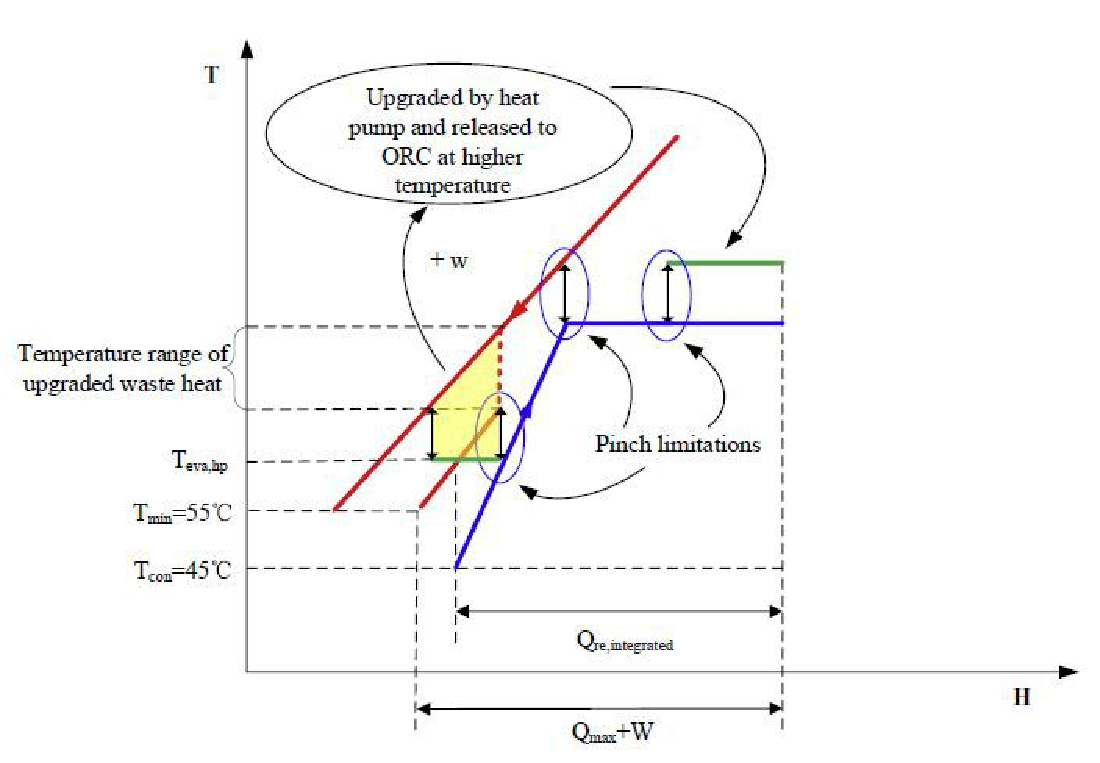
\includegraphics[scale = 0.75]{Images/PinchPoints.pdf}
  \caption{Pinch point optimised T-H diagram for the integrated ORC \parencite{YU2018330}}
  \label{fig:PinchPointOpt}
\end{figure}

\section{Methodology}
To complete the model \todo{rephrase} it is necessary to apply some simplifying assumptions, these are:
\begin{itemize}
    \item All the machinery can operate at saturated liquid and vapour limits.
    \item Negligible heat loss
    \item Negligible pressure drop
\end{itemize}

\todo[inline]{Check that these are all the parameters}
\textcite{YU2018330} use certain assumptions for the system parameters to allow for the system to be simulated. For consistency the same parameters are used. The parameters used are stated in Table \ref{tab:params} below. These parameters are used as stated for all relevant simulations unless otherwise stated.
\begin{table}[H]
  \centering
  \caption{System parameters}
  \label{tab:params}
  \begin{tabular}{lll}
    \toprule
    Parameter & Value & Unit \\
    \midrule
    $\eta_{compressor}$\nomenclature{$\eta_{compressor}$}{Isentropic efficiency of the compressor \nomunit{1}} & 0.85 & 1\\
    $\eta_{pump}$\nomenclature{$\eta_{compressor}$}{Isentropic efficiency of the pump \nomunit{1}} & 0.8 & 1\\
    $\eta_{turbine}$\nomenclature{$\eta_{compressor}$}{Isentropic efficiency of the turbine \nomunit{1}} & 0.8 & 1\\
    $FCp_{wh}$\nomenclature{$FCp_{wh}$}{Heat capacity flow rate of the waste heat \nomunit{\si{\kilo\watt\per\celsius}}} & 100 & $\si{\kilo\watt\per\celsius}$\\
    $\Delta~T_{min}$ & 10 & $\si{\celsius}$\\
    $T_{wh,in}$\nomenclature{$T_{wh,in}$}{Temperature of waste heat into the heat exchange system \nomunit{\si{\celsius}}} & 150 & $\si{\celsius}$\\
    $T_{con,orc}$\nomenclature{$T_{con,orc}$}{Temperature at the ORC condenser outlet \nomunit{\si{\celsius}}} & 45 & $\si{\celsius}$\\
    $T_{wh,out,min}$\nomenclature{$T_{wh,out,min}$}{Minimum temperature of the waste heat outlet \nomunit{\si{\celsius}}} & $T_{con,orc}$ + 10 & $\si{\celsius}$\\
    $T_{con,hp}$\nomenclature{$T_{con,hp}$}{Temperature at the heat pumo condenser outlet \nomunit{\si{\celsius}}} & $T_{eva,orc}$ + 10 & $\si{\celsius}$\\
    $X_{eva}$\nomenclature{$X_{eva}$}{Vapour quality at the evaporator outlet \nomunit{1}} & 1 & 1\\
    $X_{con}$\nomenclature{$X_{con}$}{Vapour quality at the condenser outlet \nomunit{1}} & 0 & 1\\
    \bottomrule
  \end{tabular}
\end{table}
The standalone ORC and HP systems are separately modelled. This model is obtained through defining the enthalpy states which must be a function of two state variables according to Gibbs phase rule as per Equation \ref{eq:Gibbs} where $F$ stands for the degrees of freedom, $C$ is the number of equations and $P$ is the number of phases in the mixture. The Gibbs phase rule shows that any state can be fully defined if the degrees of freedom are known.
\begin{equation}
    \label{eq:Gibbs}
    F = C - P + 2
\end{equation}
``Coolprop" uses the two degrees of freedom required as input parameters to obtain a desired state variable as an output. Tables \ref{tab:SA_ORC_states} and \ref{tab:SA_HP_states} display the chosen parameters and obtained state variables to allow for energy balance calculations. Numbering is chosen as per Figure \ref{fig:intORC} \todo[color = yellow]{Complete and include own figure} with the subscript `$s$' indicating an isentropic state. A large number of the states are defined by their known temperatures and vapour qualities ($X$) due to the assumption that all equipment operates at the saturation limits. As the pressure accross the evaporators and condensers are constant $P_{eva,orc}$\nomenclature{$P_{eva,orc}$}{Pressure in the ORC over the evaporator \nomunit{\si{\kilo\pascal}}}, $P_{con,orc}$\nomenclature{$P_{con,orc}$}{Pressure in the ORC over the condenser \nomunit{\si{\kilo\pascal}}} and $P_{con,hp}$\nomenclature{$P_{con,hp}$}{Pressure in the heat pump over the condenser \nomunit{\si{\kilo\pascal}}} are therefore used to define the states with unknown temperatures.
\subsection{Standalone ORC}
\begin{table}[H]
  \centering
  \caption{ORC state definitions.}
  \label{tab:SA_ORC_states}
  \begin{tabular}{lll}
    \toprule
    State variable & Parameter 1 & Parameter 2 \\
    \midrule
    $P_{eva,orc}$ & $T_{eva,orc}$ & $X_{eva,orc}$\\
    $P_{con,orc}$ & $T_{con,orc}$ & $X_{con,orc}$\\
    $S_{eva,orc}$ & $T_{eva,orc}$ & $X_{eva,orc}$\\
    $H_1$ & $T_{con,orc}$ & $X_{con,orc}$\\
    $H_{2,s}$ & $P_{eva,orc}$ & $S_{con,orc}$\\
    $H_3$ & $P_{eva,orc}$ & $X_{con,orc}$\\
    $H_4$ & $T_{eva,orc}$ & $X_{eva,orc}$\\
   $H_{5,s}$ & $P_{con,orc}$ & $S_{con,orc}$\\
   $T_{pump,out}$ & $H_{2,actual}$ & $P_{eva,orc}$\\ 
    \bottomrule
  \end{tabular}
\end{table}

The isentropic states are used with the efficiencies to determine what the actual states at the outlet of the pump and turbine are as per Equations \ref{eq:H2Actual} and \ref{eq:H5Actual}. The system is hereby fully defined and therefore the working fluid mass flow rate ($\Dot{m}_{orc}$)\nomenclature{$\Dot{m}_{orc}$}{Mass flow of the organic Rankine cycle fluid \nomunit{\si{\kilo\gram\per\second}}} is calculated by relating the latent heat change of the fluid to the heat change in the waste heat stream as per Equation \ref{eq:SA_mass_flow}.
\begin{equation}
    \label{eq:H2Actual}
    H_{2,actual} = \frac{H_{2,s} - H_1}{\eta_{pump}} + H_1
\end{equation}
\begin{equation}
    \label{eq:H5Actual}
    H_{5,actual} = \eta_{turbine}(H_{5,s} - H_4)+ H_4
\end{equation}
\begin{equation}
    T_{wh,out} = T_{pump,out} + \Delta~T_{min}
\end{equation}
\begin{equation}
    Q_{wh,eva1} = FCp_{wh} (T_{eva,orc} + \Delta~T_{min} - T_{wh,out})
\end{equation}
\begin{equation}
    Q_{wh,eva2} = FCp_{wh} (T_{wh,in} - T_{eva,orc} + \Delta~T_{min})
\end{equation}
\begin{equation}
    \label{eq:SA_mass_flow}
    \Dot{m}_{orc} = \frac{Q_{wh,eva2}}{H_4 - H_3}
\end{equation}
The net heat ($P_{net}$)\nomenclature{$P_{net}$}{Net power output \nomunit{\si{\kilo\watt}}} is subsequently calculated  as per Equation \ref{eq:ORC_last} by the difference in the turbine power output ($P_{turbine}$, Equation \ref{eq:SA_turbine})\nomenclature{$P_{turbine}$}{Power produced by the turbine \nomunit{\si{\kilo\watt}}} and pump power requirement ($P_{pump}$, Equation \ref{eq:SA_pump})\nomenclature{$P_{pump}$}{Power requirement of the pump \nomunit{\si{\kilo\watt}}}.
\begin{equation}
\label{eq:SA_pump}
    P_{pump} = \Dot{m}_{orc} |H_{2,actual} - H_1|
\end{equation}
\begin{equation}
\label{eq:SA_turbine}
    P_{turbine} = \Dot{m}_{orc} |H_{5,actual} - H_4|
\end{equation}
\begin{equation}
    Q_{wh,rec} = \Dot{m}_{orc} |H_4 - H_{2,actual}|
\end{equation}
\begin{equation}
    \label{eq:ORC_last}
    P_{net} = P_{turbine} - P_{pump}
\end{equation}
\subsection{Standalone Heat Pump}
\begin{table}[H]
  \centering
  \caption{Heat pump state definitions.}
  \label{tab:SA_HP_states}
  \begin{tabular}{lll}
    \toprule
    State variable & Parameter 1 & Parameter 2 \\
    \midrule
    $P_{con,hp}$ & $T_{con,hp}$ & $X_{con,hp}$\\
    $S_{eva,hp}$ & $T_{eva,hp}$ & $X_{eva,hp}$\\
    $H_{I}$ & $T_{con,hp}$ & $X_{con,hp}$\\
    $H_{II}$ & $T_{eva,hp}$ & $X_{eva,hp}$\\
    $H_{III,s}$ & $P_{con,hp}$ & $S_{eva,hp}$\\
    \bottomrule
  \end{tabular}
\end{table}
Similar to the ORC the enthalpic states of the heat pump are defined in Table \ref{tab:SA_HP_states}. The use of a throttle valve implies that the enthalpies on both sides of the valve are equal \parencite{SmithVanNessAbbott}, as stated in Equation \ref{eq:SA_HP_H4}.  The isentropic enthalpy is used in conjunction with the thermal efficiency the compressor to find the actual value of the enthalpy for the exit of the compressor from Equation \ref{eq:SA_HP_H3actual}. From the enthalpic states the heat out of the heat pump and the compressor work requirement are calculated as per Equations \ref{eq:SA_HP_Qout} and \ref{eq:SA_HP_W} respectively.
\begin{equation}
    \label{eq:SA_HP_H4}
    H_{IV} = H_{I}
\end{equation}
\begin{equation}
    \label{eq:SA_HP_H3actual}
    H_{III,actual} = \frac{H_{III,s} - H_{II}}{\eta_{compressor}} + H_{II}
\end{equation}
\begin{equation}
    \label{eq:SA_HP_Qout}
    Q_{out,hp} = H_{IV} - H_{III,actual}
\end{equation}
\begin{equation}
    \label{eq:SA_HP_W}
    W_{hp} = H_{III,actual} - H_{II}
\end{equation}
\subsection{Integrated Organic Rankine Cycle and Heat Pump}
The discussion that follows is a simplified version of the necessary equations. Consult \textcite{YU2018330} for the complete equation set. 

The ratio of the latent to the sensible heat ($r_l/s$)\nomenclature{$r_l/s$}{ ratio of latent to sensible heat \nomunit{1}} is calculated as per Equation \ref{eq:rls}. This ratio is constant under constant fixed evaporation and condensation temperatures. $R_l$\nomenclature{$R_l$}{Molar latent heat \nomunit{\si{\joule\per\mole}}}, $R_s$\nomenclature{$R_s$}{Molar sensible heat \nomunit{\si{\joule\per\mole}}}, $Q_l$\nomenclature{$Q_l$}{Total latent heat \nomunit{\si{\joule\per\mole}}} and $Q_s$\nomenclature{$Q_s$}{Total latent heat \nomunit{\si{\joule\per\mole}}} represent molar latent heat, molar sensible heat, total latent heat and total sensible heat respectively.
\begin{equation}
    \label{eq:rls}
    r_{l/s} = \frac{R_l}{R_s} = \frac{Q_l}{Q_s} = Constant
\end{equation}
The ratio $r_{l/s}$ is used to cancel out the ratios of sensible heat up until the cliff temperature to the latent and total sensible heat, this is necessary due limitation created by the unknown cliff temperature . The combination and simplification of these individual equations, their associated energy calculations, an overall energy balance and Equation \ref{eq:COP} results in Equation \ref{eq:QinHP2}.
\begin{equation}
    \label{eq:QinHP2}
    Q_{in,hp} = \frac{FCp_{wh}[(T_{eva,orc} - T_{con,orc})R_{l/s} - (T_{in,wh} - T_{eva,orc} - \Delta~T_{min})]}{R_{l/s}(T_{eva,orc} - T_{con,orc}/(T_{eva,orc} - T_{eva,hp}) + [COP/(COP - 1)]}
\end{equation}
The COP is used as per Equation \ref{eq:COP} and combined with the overall system energy balance to obtain a description for the heat pump work requirement as given in Equation \ref{eq:Whp}. It is worthy to note that \textcite{YU2018330} incorrectly state this equation in their published report (Equation 8 in \textcite{YU2018330}).
\begin{equation}
    \label{eq:Whp}
    W_{hp} = Q_{in,hp}/(COP - 1)
\end{equation}
The temperature at which the waste heat is upgraded by the heat pump is known as the cliff temperature ($T_{cliff}$)\nomenclature{$T_{cliff}$}{Temperature cliff \nomunit{\si{\celsius}}}. This temperature is calculated as per Equation \ref{eq:Tcliff} below. The heat capacity flow rate ($FCp_{orc}$)\nomenclature{$FCp_{orc}$}{Heat capacity flow rate of the ORC \nomunit{\si{\kilo\watt\per\celsius}}} of the ORC is found through relating the energy difference of the waste heat to heat change of the ORC due to the waste heat. This is shown in Equation \ref{eq:FCporc}.
\begin{equation}
    \label{eq:Tcliff}
    T_{cliff} = T_{eva,hp} + \Delta~T_{min} + Q_{in,hp}/FCp_{wh}
\end{equation}
\begin{equation}
    \label{eq:FCporc}
    FCp_{orc} = \frac{FCp_{wh}(T_{eva,orc} + \Delta~T_{min} - T_{cliff})}{T_{eva,orc} - T_{eva,hp}}
\end{equation}
The total sensible heat of the ORC is calculated by multiplying the temperature difference between the evaporation and condensation temperature with the heat capacity flow rate. The unrecovered waste heat ($Q_{wh,unre}$)\nomenclature{$Q_{wh,unre}$}{Unrecovered waste heat \nomunit{\si{\kilo\watt}}} is calculated from the difference in the maximum possible waste heat and the total ORC sensible heat as per Equation \ref{eq:Qwhunre}.
\begin{equation}
    \label{eq:Qwhunre}
    Q_{wh,unre} = FCp_{orc}(T_{eva,orc} +\Delta~T_{min} - T_{cliff} + T_{eva,hp} + \Delta~T_{min} - T_{out,wh,min}) - Q_{orc,s}
\end{equation}
Equation \ref{eq:Toutwh} shows the outlet temperature of the waste heat ($T_{out,wh}$)\nomenclature{$T_{out,wh}$}{Waste heat outlet temperature \nomunit{\si{\celsius}}} is calulated by adding the effect of the waste heat unrecovered to the minimum outlet waste heat.
\begin{equation}
    \label{eq:Toutwh}
    T_{out,wh} = T_{out,wh,min} + Q_{wh,unre}/FCp_{wh}
\end{equation}
The waste heat which is captured ($Q_{wh,re}$)\nomenclature{$Q_{wh,re}$}{Waste heat recovered \nomunit{\si{\kilo\watt}}} is calculated from the maximum heat, the work into the heat pump and then subtracting the unrecovered heat as per Equation \ref{eq:Qwhre}. This is used in combination with the thermal efficiency to determine the ORC power and subsequently the net power output from Equations \ref{eq:Porc} and \ref{eq:Pnet}.
\begin{equation}
    \label{eq:Qwhre}
    Q_{wh,re} = FCp_{wh}(T_{in,wh} - T_{out,wh,min}) + W_{hp} - Q_{wh,unre}
\end{equation}
\begin{equation}
    \label{eq:Porc}
    P_{orc} = \eta~Q_{wh,re}
\end{equation}
\begin{equation}
    \label{eq:Pnet}
    P_{net} = P_{orc} - W_{hp}
\end{equation}

\section{Results and Discussion}
\todo[inline, color = cyan]{Discuss COP comparative performance}

 \begin{figure}[H]
  \centering
  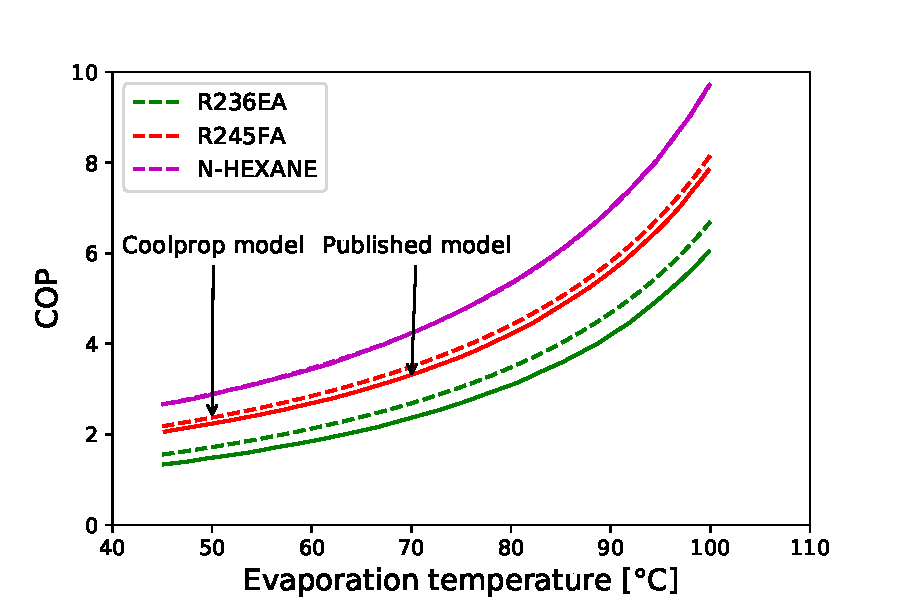
\includegraphics[scale = 0.65]{Images/COP_HP_SA.pdf}
  \caption{Comparison of COP for different fluids between \cite{YU2018330} (solid~lines) and ``Coolprop" (serrated lines) models at a constant condensation temperature (\SI{130}{\celsius}).}\label{fig:COP_SA}
  
  \todo[inline, color = cyan]{Discuss SA ORC comparative performance}
  \todo[inline,color= yellow]{Check ordering of COP and SA ORC eq,s and graphs}
\end{figure}
\begin{figure}[H]
    \begin{subfigure}[l]{1\textwidth}
      \centering
      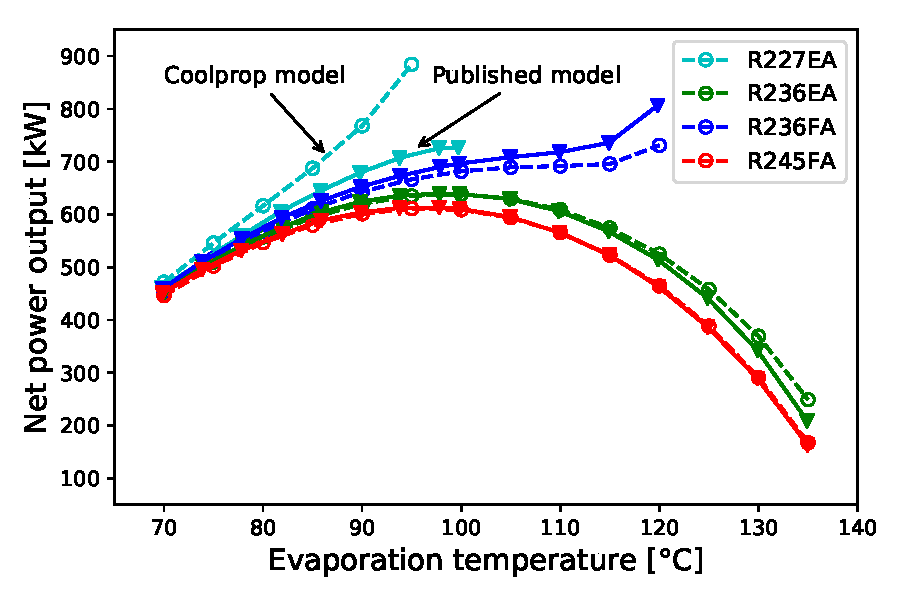
\includegraphics[scale = 0.65]{Images/ORC_PNET_SA.pdf}
      \caption{Net power output}\label{fig:ORC_PNET_SA}
    \end{subfigure}
    \begin{subfigure}[l]{1\textwidth}
      \centering
      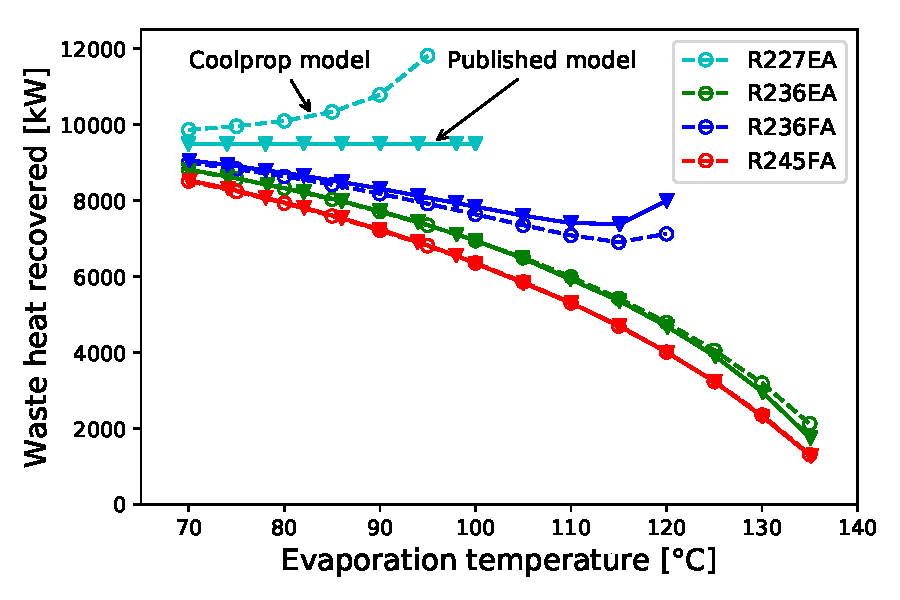
\includegraphics[scale = 0.69]{Images/ORC_WH_REC_SA.pdf}
      \caption{Waste heat recovered}
      \label{fig:ORC_WH_REC_SA}
     \end{subfigure}
    \label{fig:ORC_SA}
    \caption{Comparison between standalone ORC system performance between \cite{YU2018330} (solid~lines) and ``Coolprop" (serrated~lines) models.}
\end{figure}
\todo[inline]{From this point on need confirmation that graphs are correct before continuing}
\todo[inline, color = cyan]{Include table of Comparative optimal results}
 \begin{figure}[H]
  \centering
  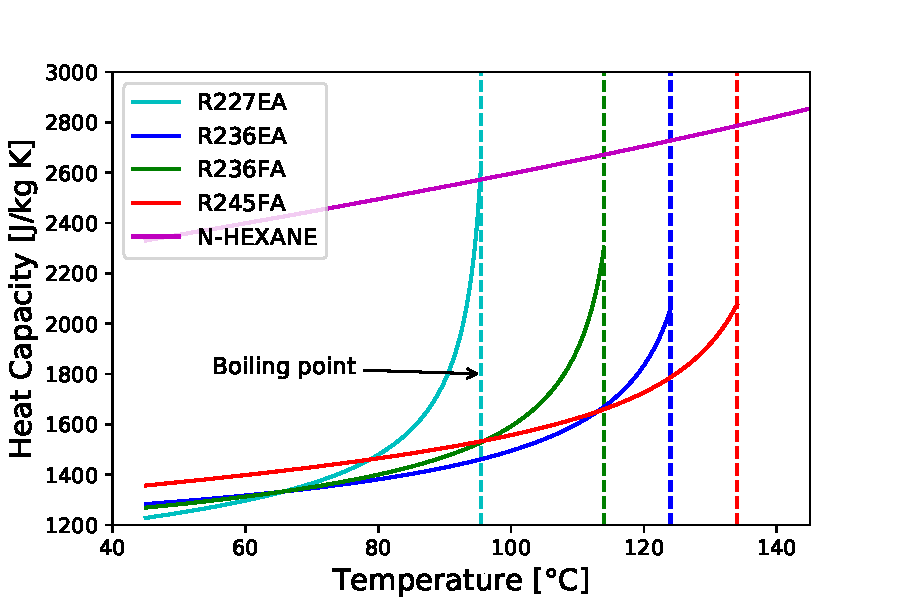
\includegraphics[scale = 0.65]{Images/CP.pdf}
  \caption{Heat Capacity variation with temperature for different working fluids with serrated lines indicating boiling points.}
  \label{fig:CP}
\end{figure}
 \begin{figure}[H]
  \centering
  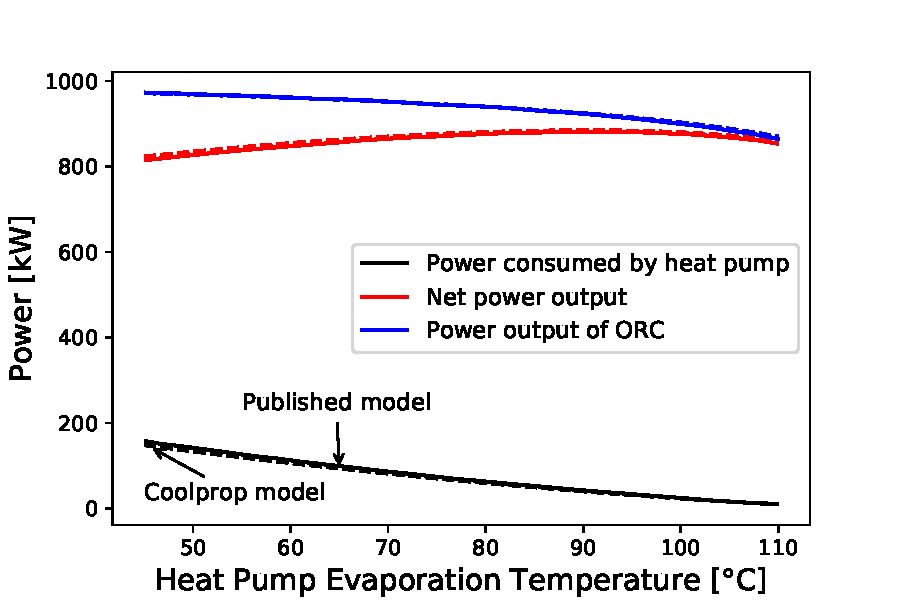
\includegraphics[scale = 0.65]{Images/Int_R236FA.pdf}
  \caption{Comparison of Integrated system performance between \cite{YU2018330} (solid~lines) and ``Coolprop" (serrated~lines) models using R236FA as the ORC working fluid.}
  \label{fig:IntR236FA}
\end{figure}
\begin{figure}[H]
   \begin{subfigure}[H]{.32\textwidth}
      \centering
      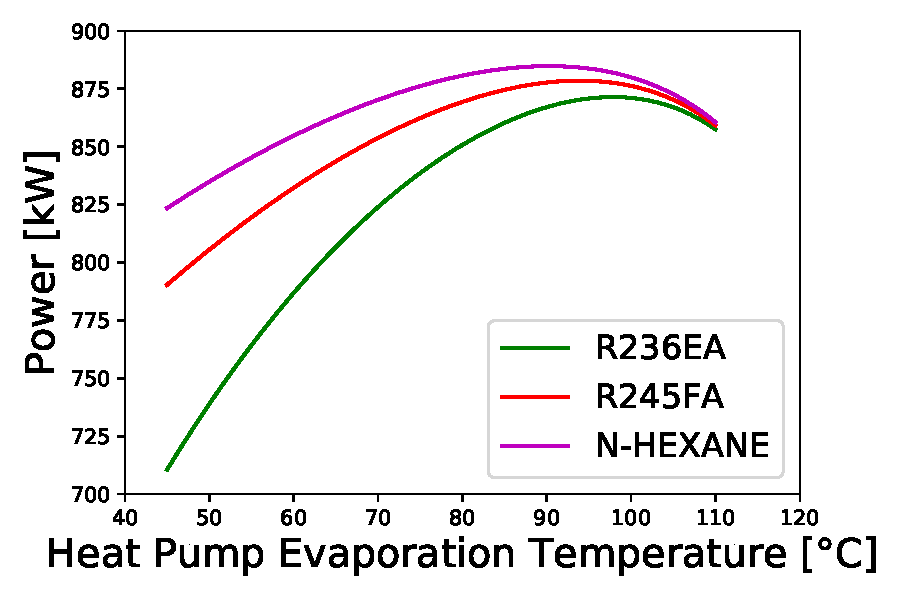
\includegraphics[scale = 0.35]{Images/P_NET_FLUIDS_HP.pdf}
      \caption{Net Power Output}
      \label{fig:P_NET_HP}
    \end{subfigure}
    \begin{subfigure}[H]{.32\textwidth}
      \centering
      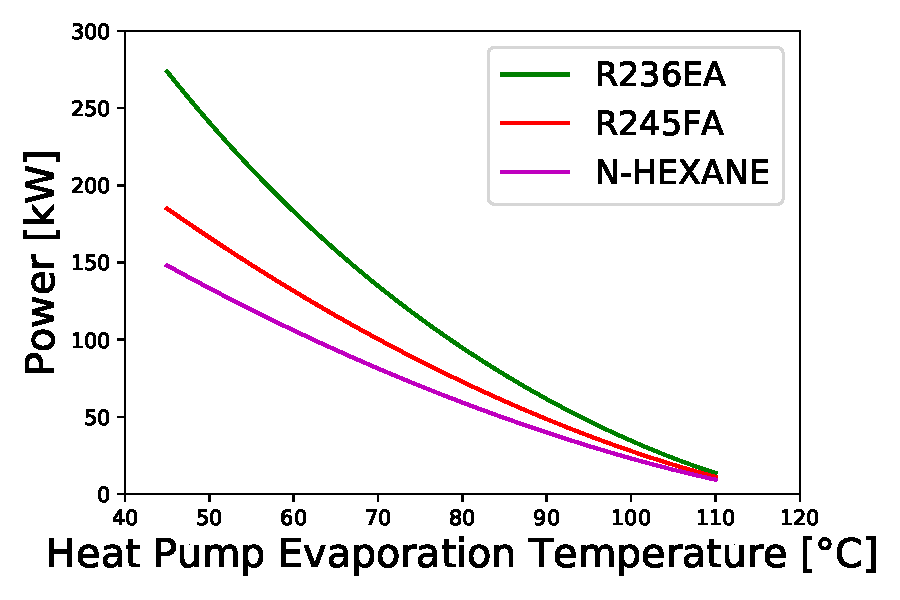
\includegraphics[scale = 0.35]{Images/P_HP_FLUIDS_HP.pdf}
      \caption{Power consumed by HP}
      \label{fig:P_HP_HP}
    \end{subfigure}
    \begin{subfigure}[H]{.32\textwidth}
      \centering
      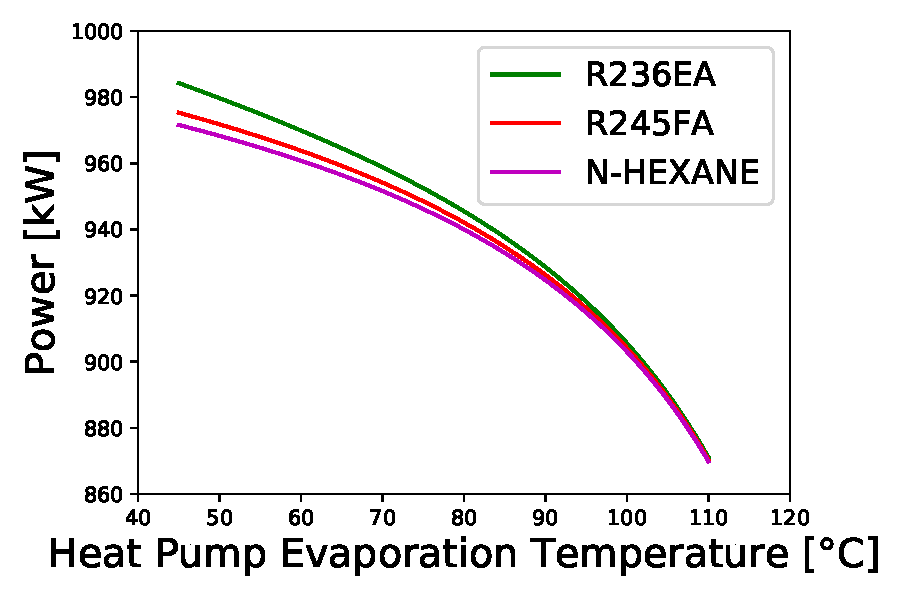
\includegraphics[scale = 0.35]{Images/P_ORC_FLUIDS_HP.pdf}
      \caption{Power output of ORC}
      \label{fig:P_ORC_HP}
    \end{subfigure}
\caption{Integrated system performance of different heat pump working fluids with R236FA as the ORC working fluid.}
\label{fig:Fluids_HP}
\end{figure}
\begin{figure}[H]
   \begin{subfigure}[H]{.32\textwidth}
      \centering
      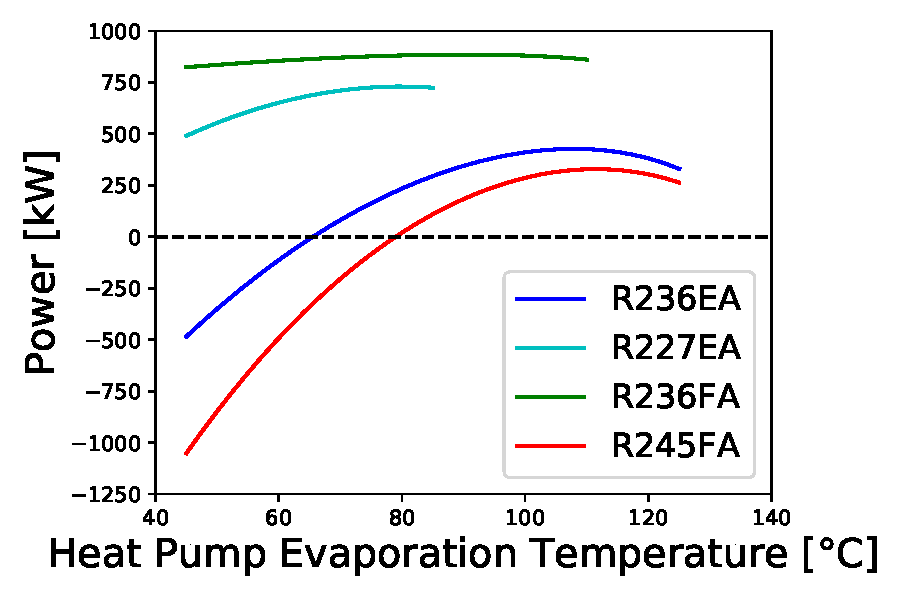
\includegraphics[scale = 0.35]{Images/P_NET_FLUIDS_ORC.pdf}
      \caption{Net Power Output}
      \label{fig:P_NET_ORC}
    \end{subfigure}
    \begin{subfigure}[H]{.32\textwidth}
      \centering
      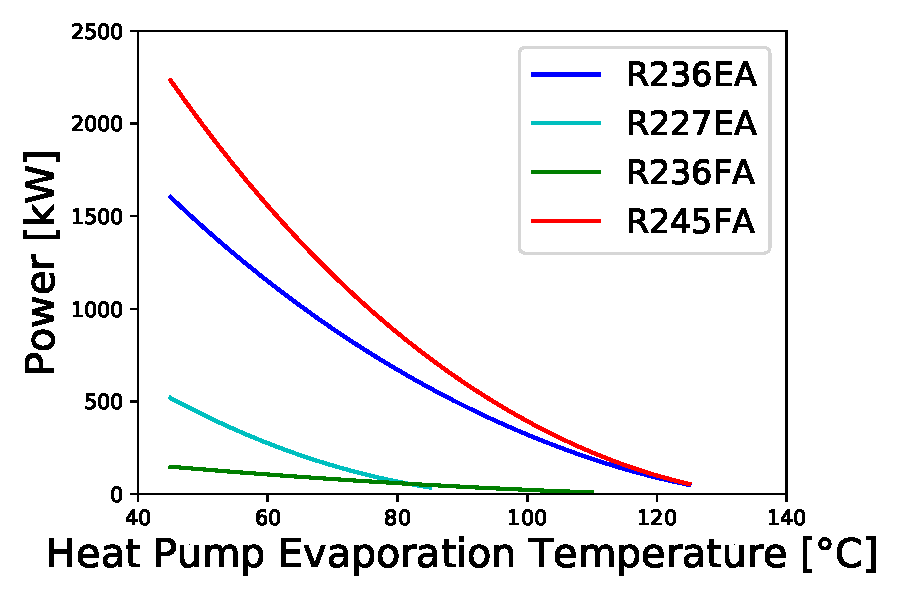
\includegraphics[scale = 0.35]{Images/P_HP_FLUIDS_ORC.pdf}
      \caption{Power consumed by HP}
      \label{fig:P_HP_ORC}
    \end{subfigure}
    \begin{subfigure}[H]{.32\textwidth}
      \centering
      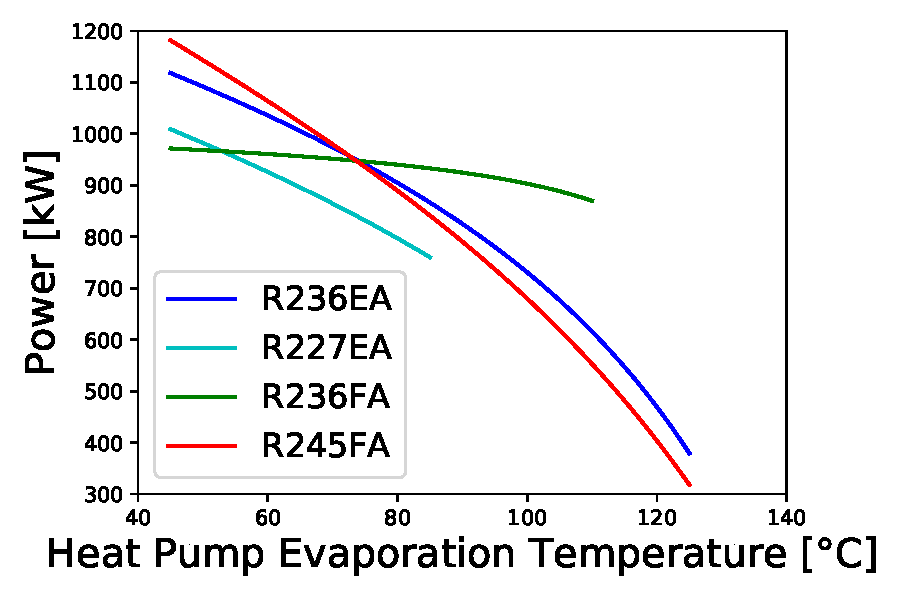
\includegraphics[scale = 0.35]{Images/P_ORC_FLUIDS_ORC.pdf}
      \caption{Power output of ORC}
      \label{fig:P_ORC_ORC}
    \end{subfigure}
\caption{Integrated system performance of different ORC working fluids with N-Hexane as the ORC working fluid.}
\label{fig:Fluids_ORC}
\end{figure}

Discussion topics
\begin{itemize}
    \item Tabulated comparison of optimal conditions
    \item Constant CP assumption
    \item Other fluids
    \item Usefulness as a waste heat recovery tool
\end{itemize}



\newpage

\begin{equation}
    H1 = f(T_{con},Q_{con})
\end{equation}
\begin{equation}
    H2 = f(T_{eva},Q_{con})
\end{equation}
\begin{equation}
    H3 = f(T_{eva},Q_{eva})
\end{equation}
\begin{equation}
    R_S = H2 - H1
\end{equation}
\begin{equation}
    R_L = H3 - H2
\end{equation}
\begin{equation}
    R_{ls} = R_L/R_S
    \label{eq:fig}
\end{equation}
\begin{equation}
    \label{eq:ThermalEffec1}
    \eta_T = \frac{|W|}{|Q_H|}
\end{equation}
\begin{figure}[H]
  \centering
  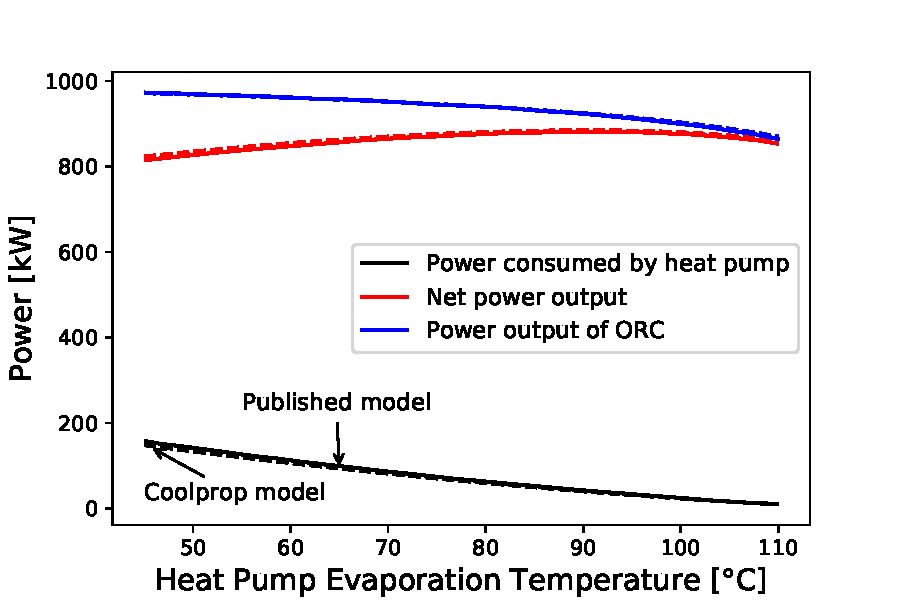
\includegraphics[scale = 0.65]{Images/Int_R236FA.pdf}
  \caption{Original (with published heat ratio and thermal efficiency) integrated system performance of different heat pump working fluids with R236FA as the ORC working fluid.}\label{fig:Int}
\end{figure}
\begin{figure}[H]
  \centering
  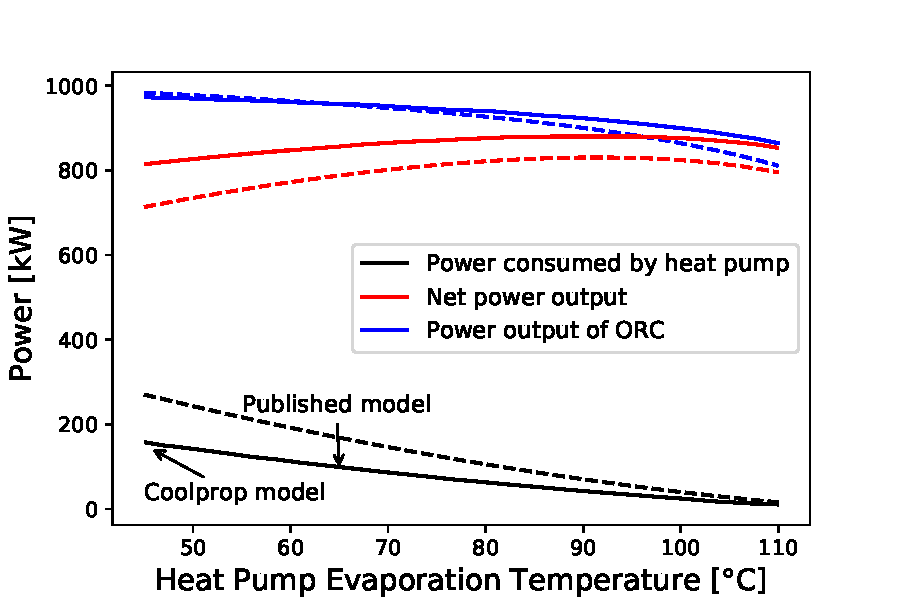
\includegraphics[scale = 0.65]{Images/Int_R236FA_rls.pdf}
  \caption{Performance with $R_{ls}$ calculated as per Equation \ref{eq:fig} with enthalpy states}\label{fig:Int_rls}
\end{figure}
\begin{figure}[H]
  \centering
  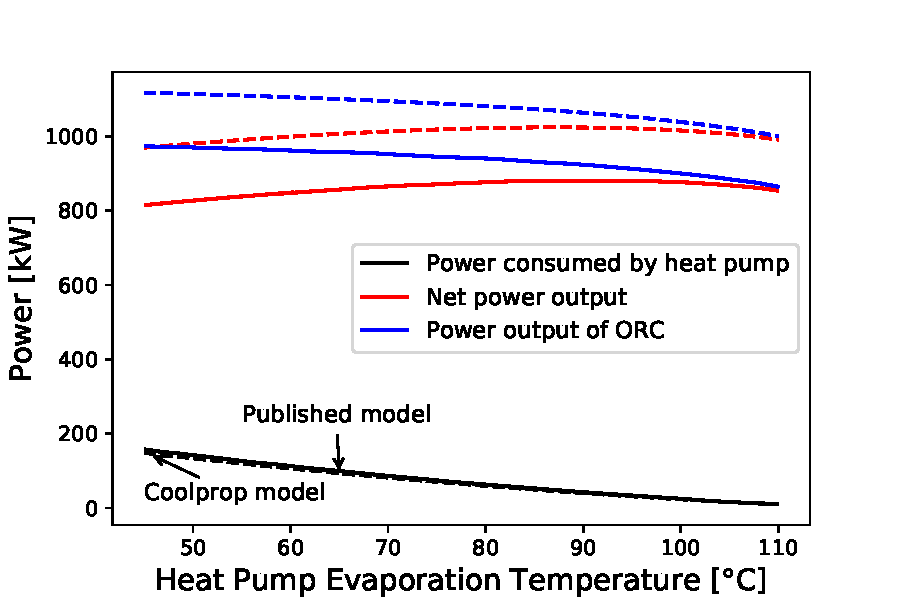
\includegraphics[scale = 0.65]{Images/Int_R236FA_eta.pdf}
  \caption{Performance with $\eta$ calculated as per Equation \ref{eq:ThermalEffec1} with enthalpy states}\label{fig:Int_eta}
\end{figure}
The work and heat into the system are found using the defined enthalpy states of the overall system. The ratio of latent to sensible heat is also found using enthalpy states from coolprop. The efficiency and $r_{ls}$ are always higher than the published versions. 
\begin{figure}[H]
  \centering
  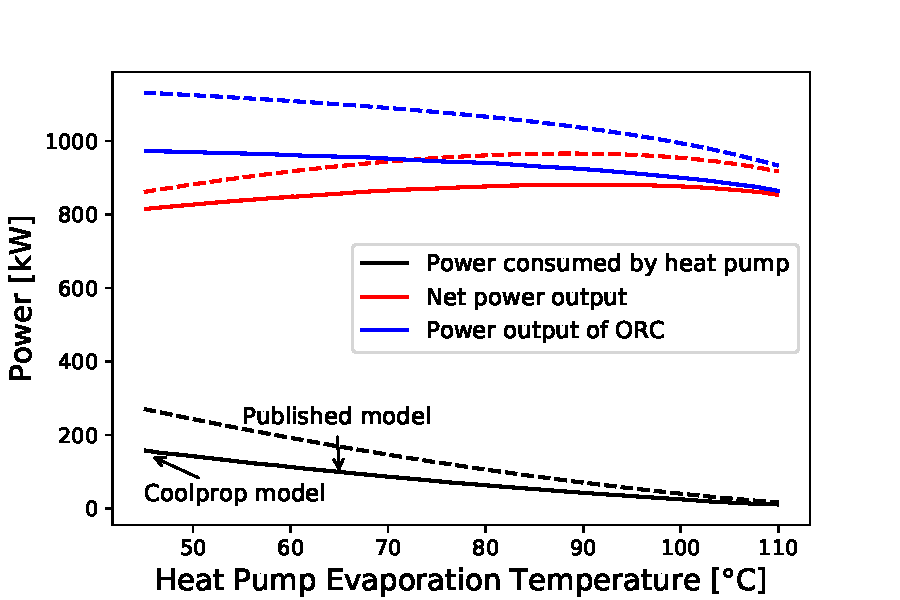
\includegraphics[scale =0.65]{Images/Int_R236FA_both.pdf}
  \caption{Performance with both $\eta$ and $R_{ls}$ calculated with enthalpy states}\label{fig:Int_both}
\end{figure}
I expect that either there is a coding error or Coolprop's enthalpies are different to that of Aspen. The discussion approach would be to further investigate $R_S$ calculating it from another approach to check the enthalpy values against. If this proves correct then this would show an inconsistency between the published and Coolprop modelled results. As the results using the published efficiency and heat ratio, this shows the difference must be due to these two parameters. It may be necessary to again critically evaluate the accuracy of these parameters.

\newpage
\section{Conclusion and Recommendations}

\printbibliography

\listoftodos
\end{document}